\documentclass[a4j]{jarticle}

%% 使用するパッケージ
\usepackage{listings}
\usepackage[]{graphicx}
\usepackage[dvipdfmx]{color}
\usepackage{amssymb}
\usepackage[]{multicol}
\usepackage{url}
\西暦

%% 表紙
\title{FAT32解説小冊子}
\author{feynoobs}
\begin{document}

\maketitle

\begin{abstract}
本冊子では仮想マシン2台を使用したC言語によるFreeBSDのKernelのデバッグ方法を示す。
なお、Bootのごく先頭部分はKernelデバッグできない。

\end{abstract}
\begin{multicols}{2}

\section{環境準備}
ホストのPCにUbuntu15.10を使用した場合の環境構築手順を示す。
\ref{tb:FreeBSD:_ENV}に示すのアプリケーションがインストール
されていることを前提で話をすすめる。
\begin{table*}[htp]
	\caption{必要なアプリケーション}
	\label{tb:FreeBSD:_ENV}
	\begin{center}
		\begin{tabular}{l|p{10cm}}										\hline
			アプリケーション	&	概要							\\	\hline
			QEMU				&	x64エミュレータ				\\	\hline	\hline
			OVMF.fd				&	UEFIイメージ					\\	\hline	\hline
			FreeBSDイメージ		&	AMD64・UEFI対応のFreeBSDのISO	\\	\hline
		\end{tabular}
	\end{center}
\end{table*}

\section{環境構築}
\subsection{FreeBSDインストール}
\label{sec:FreeBSD_inst}
\ref{fig:FreeBSD_CREATE}の操作でFreBSDをインストールする仮想ディスクを作成する。
\begin{figure*}[htbp]
	\begin{center}
  		\begin{lstlisting}[basicstyle=\ttfamily\footnotesize, frame=single, breaklines=true]
$ qemu-img create -f qcow2 GUEST1 16G
  		\end{lstlisting}
	\end{center}
	\caption{FreeeBSDを格納するファイルシステム作成}
	\label{fig:FreeBSD_CREATE}
\end{figure*}

\ref{fig:FreeBSD_QEMU}の操作でFreeBSDをインストール開始する。
\begin{figure*}[htbp]
	\begin{center}
		\begin{lstlisting}[basicstyle=\ttfamily\footnotesize, frame=single, breaklines=true]
$ qemu-system-x86_64 -enable-kvm -bios OVMF.fd -hda GUEST1  -cdrom FreeBSD-10.2-RELEASE-amd64-uefi-disc1.iso -m 1024M -smp 2
		\end{lstlisting}
	\end{center}
	\caption{FreeBSDをインストールするためのQEMU起動}
	\label{fig:FreeBSD_QEMU}
\end{figure*}

QEMUを起動してしばらく経つと\ref{fig:FreeBSD_TOP}の画面になるので
``$<$Install$>$''を選択する。
\begin{figure*}[htbp]
	\begin{center}
    	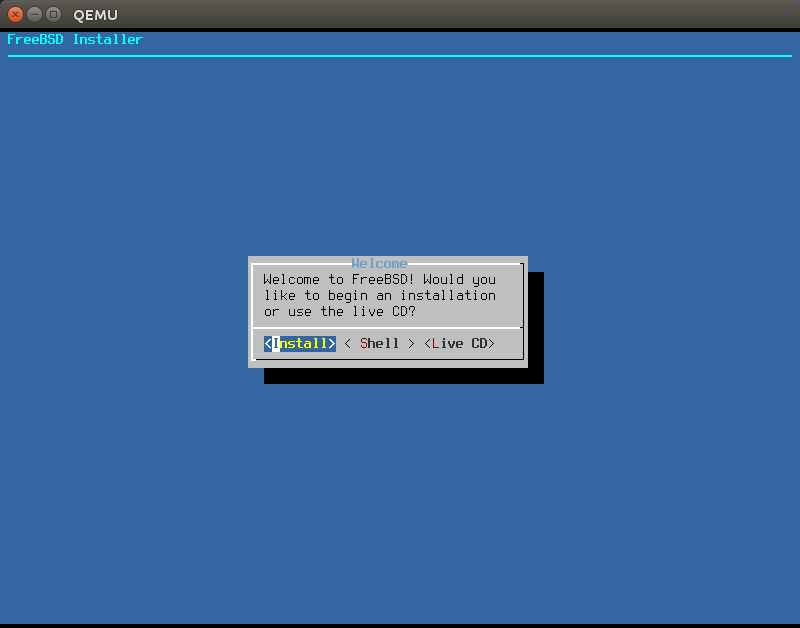
\includegraphics[width=10cm]{./IMG/FreeBSD_TOP.png}
	\end{center}
    \caption{インストーラの初期画面}
    \label{fig:FreeBSD_TOP}
\end{figure*}

\ref{fig:FreeBSD_KEY}のキーマップ選択画面はPCのキー配置にしたがって選択する。
日本語キーボードの場合は"Japanses 106"で良いであろう。
選択したあと``$>>>$Continue with jp.106.kdb keymap''を選択する。
\begin{figure*}[htbp]
	\begin{center}
    	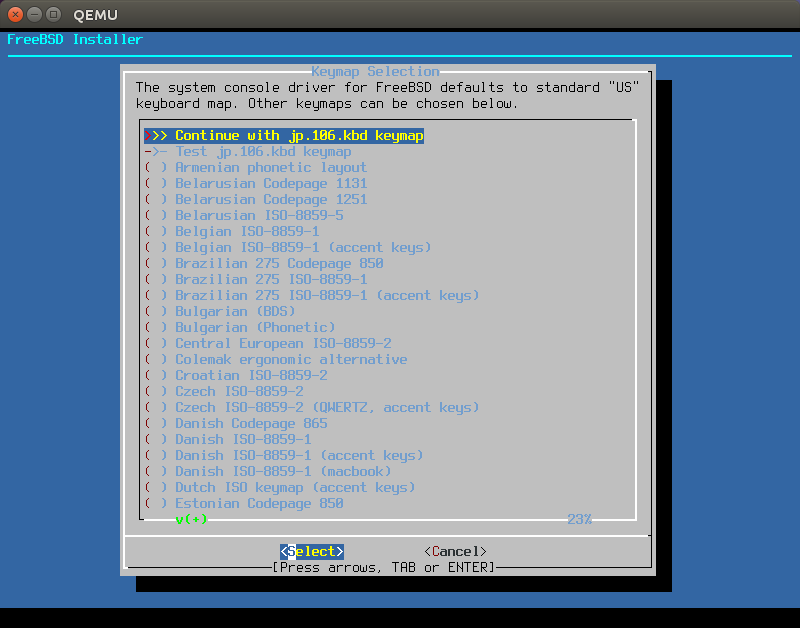
\includegraphics[width=10cm]{./IMG/FreeBSD_JP106.png}
	\end{center}
    \caption{キーマップ選択画面}
    \label{fig:FreeBSD_KEY}
\end{figure*}

\ref{fig:FreeBSD_HOST}のHOST名は任意の名前でよい。
筆者は``feynoobs''とした。
\begin{figure*}[htbp]
	\begin{center}
    	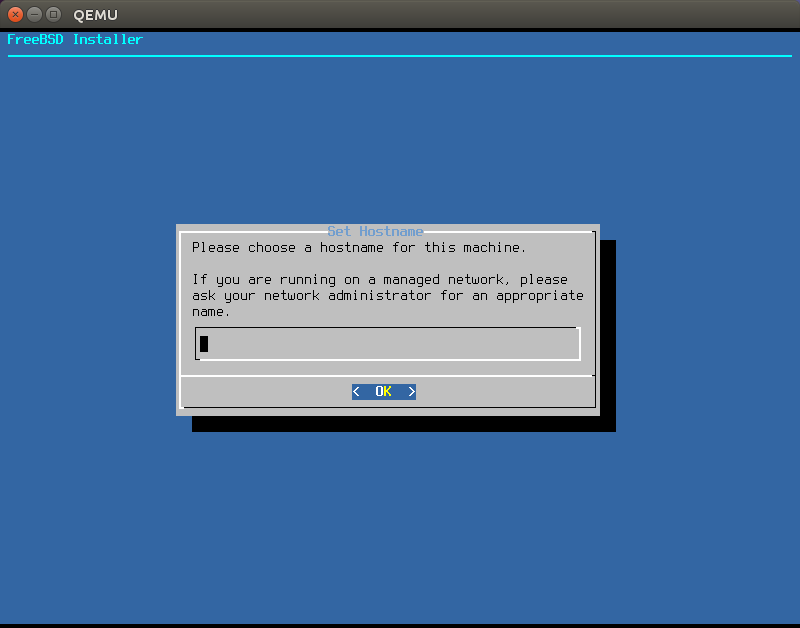
\includegraphics[width=10cm]{./IMG/FreeBSD_HOST.png}
	\end{center}
    \caption{ホスト名設定画面}
    \label{fig:FreeBSD_HOST}
\end{figure*}

\ref{fig:FreeBSD_INST_SELECT}にて"lib32"と"src"にチェックを入れて確定する。
なお、portsはユーザーとしてFreeBSDを使うときは必須であるが、デバッガとして使う場合は任意である。
\begin{figure*}[htbp]
	\begin{center}
    	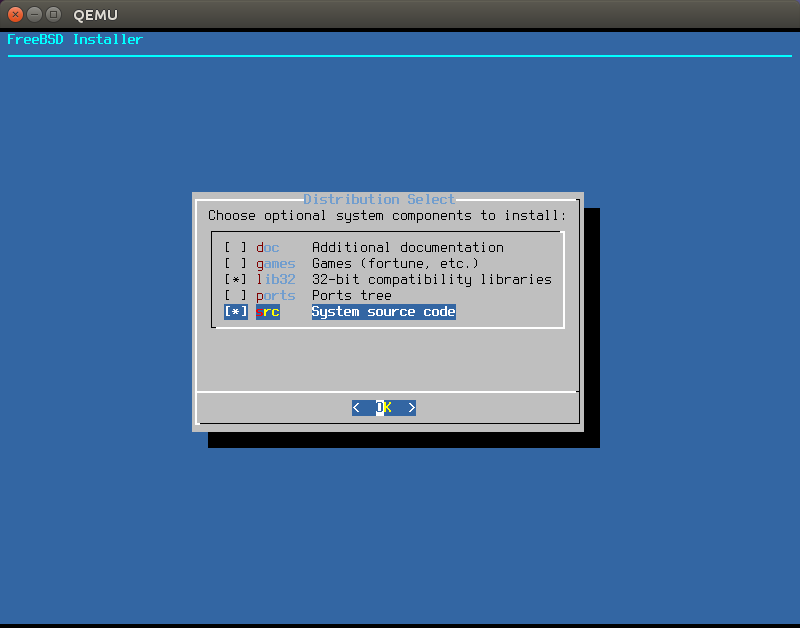
\includegraphics[width=10cm]{./IMG/FreeBSD_INST.png}
	\end{center}
    \caption{インストールする対象物}
    \label{fig:FreeBSD_INST_SELECT}
\end{figure*}

\ref{fig:FreeBSD_FS}でFreeBSDで使用するファイルシステムを選択する。
通常は``Auto(UFS)''で良い。
\begin{figure*}[htbp]
	\begin{center}
    	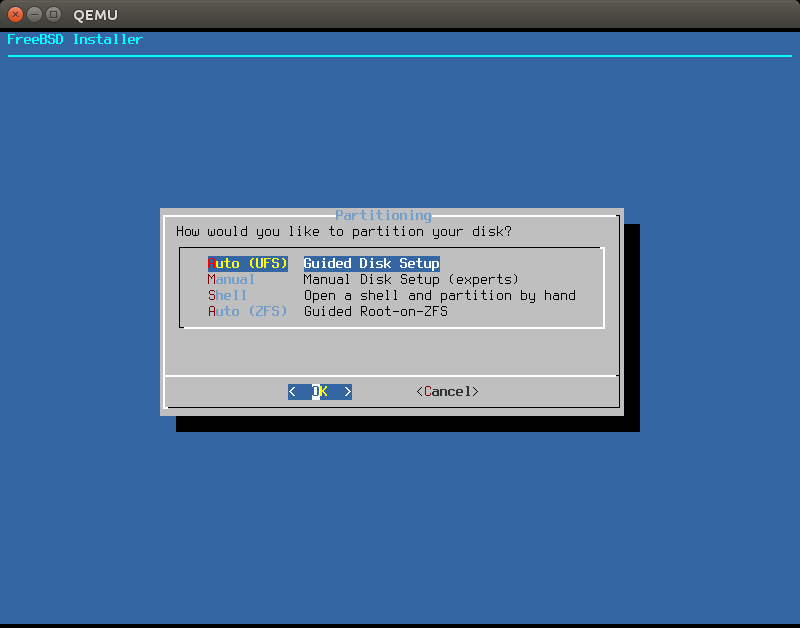
\includegraphics[width=10cm]{./IMG/FreeBSD_AUTO.png}
	\end{center}
    \caption{FreeBSDで使用するファイルシステム}
    \label{fig:FreeBSD_FS}
\end{figure*}

この仮想マシンにはFreeBSD以外のOSはインストールしないため
\ref{fig:FreeBSD_Q}``$<$Entire Dsik$>$''でよい。
\begin{figure*}[htbp]
	\begin{center}
    	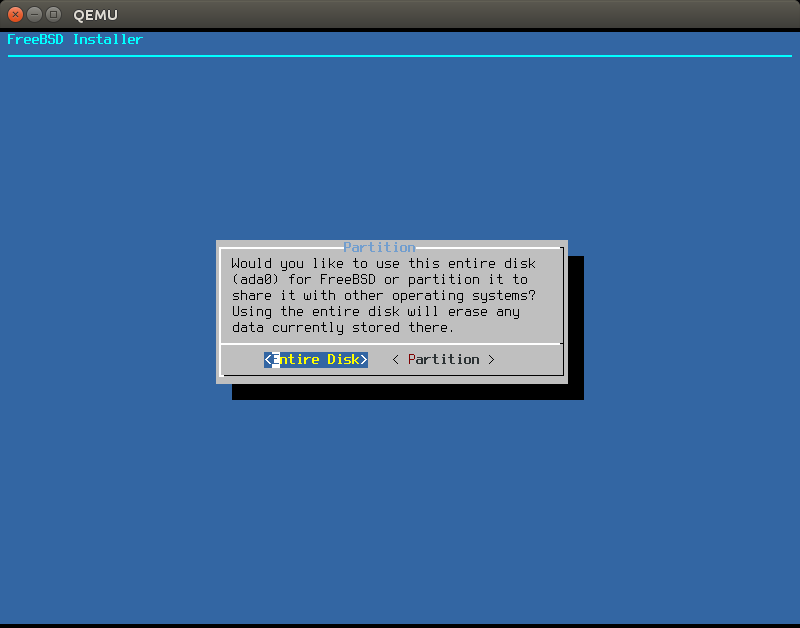
\includegraphics[width=10cm]{./IMG/FreeBSD_ENTRY.png}
	\end{center}
    \caption{QEMUでUEFIアプリケーション実行3}
    \label{fig:FreeBSD_Q}
\end{figure*}

\ref{fig:FreeBSD_GPT}はストレージ管理を"MBR"で行うか"GPT"で行うかを選択する画面である。
他の管理方法はほとんど使われていないので無視する。
ここではUEFIらしく``MBR''より優れた``GPT''を選択しています。
\begin{figure*}[htbp]
	\begin{center}
    	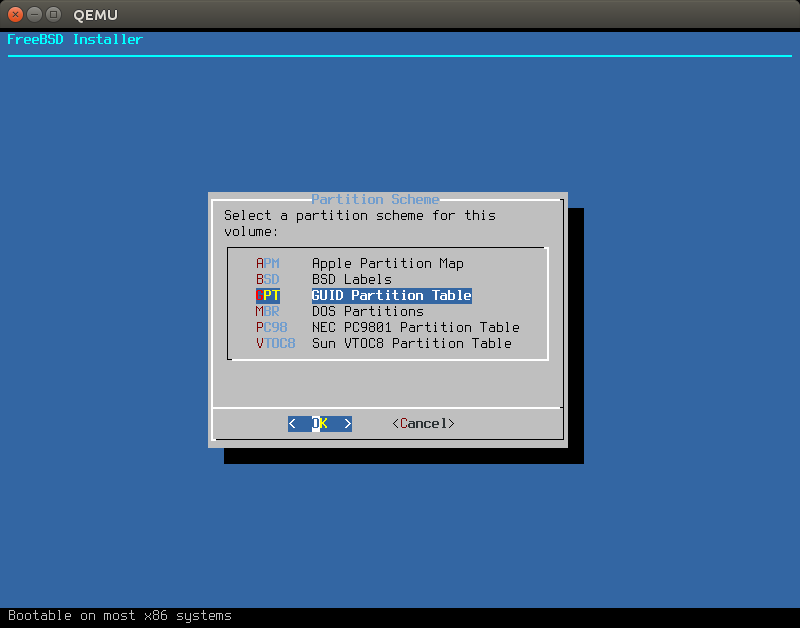
\includegraphics[width=10cm]{./IMG/FreeBSD_GPT.png}
	\end{center}
    \caption{ストレージ管理の方式}
    \label{fig:FreeBSD_GPT}
\end{figure*}

\ref{fig:FreeBSD_FileSYstem_fin}で``$<$Finish$>$''を選択すると、
\ref{fig:FreeBSD_FileSYstem_com}が表示されるので``$<$Commit$>$''する。
\begin{figure*}[htbp]
	\begin{center}
    	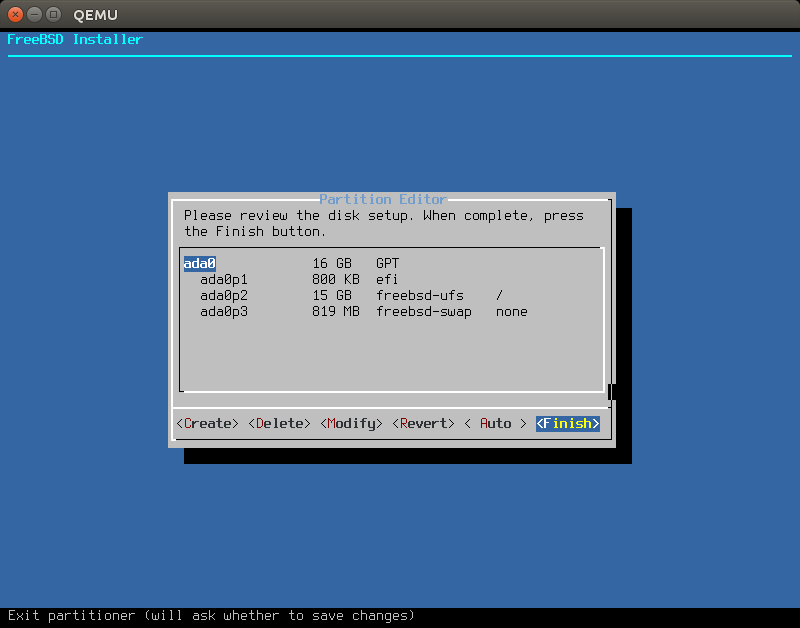
\includegraphics[width=10cm]{./IMG/FreeBSD_PT_FIX.png}
	\end{center}
    \caption{ファイルシステム確定}
    \label{fig:FreeBSD_FileSYstem_fin}
\end{figure*}
\begin{figure*}[htbp]
	\begin{center}
    	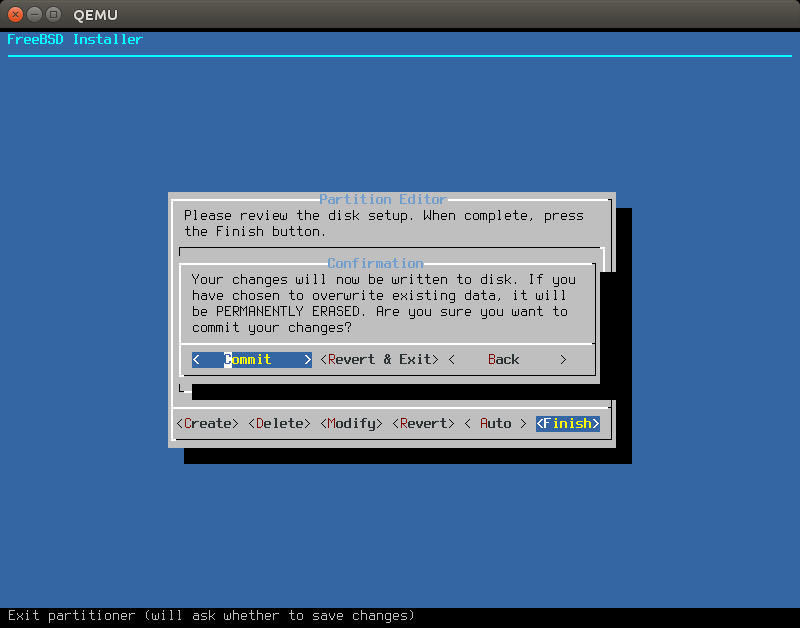
\includegraphics[width=10cm]{./IMG/FreeBSD_COMMIT.png}
	\end{center}
    \caption{ファイルシステムコミット}
    \label{fig:FreeBSD_FileSYstem_com}
\end{figure*}

インストール作業が終わると\ref{fig:FreeBSD_PASS}の画面でrootのパスワードを設定する。
パスワードを設定したくない場合はそのままエンターキーを押下する。
\begin{figure*}[htbp]
	\begin{center}
    	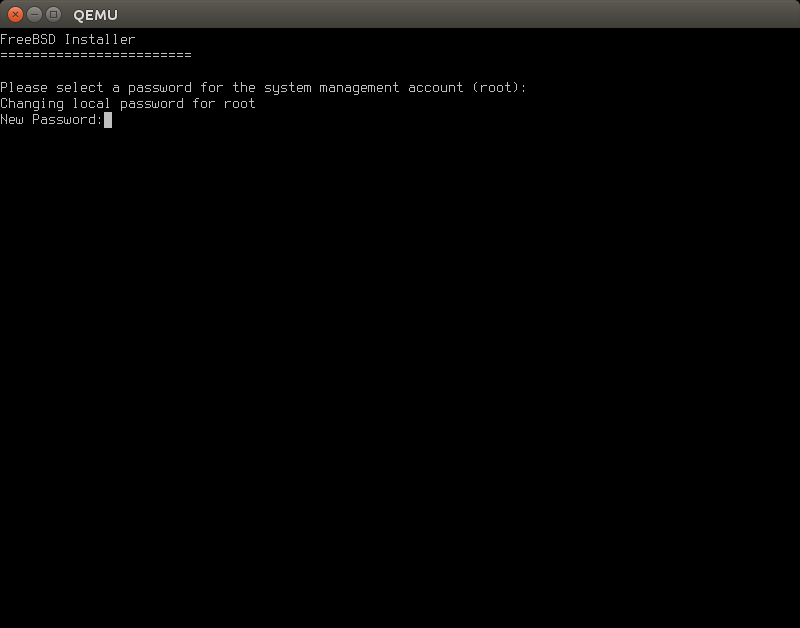
\includegraphics[width=10cm]{./IMG/FreeBSD_ROOT_PASS.png}
	\end{center}
    \caption{パスワード設定画面}
    \label{fig:FreeBSD_PASS}
\end{figure*}

\ref{fig:FreeBSD_NIC}のようなNIC設定の画面が表示される。
筆者は設定なかったので``$<$Cancel$>$''を選択した。
ネットワークの設定は割愛する。
\begin{figure*}[htbp]
	\begin{center}
    	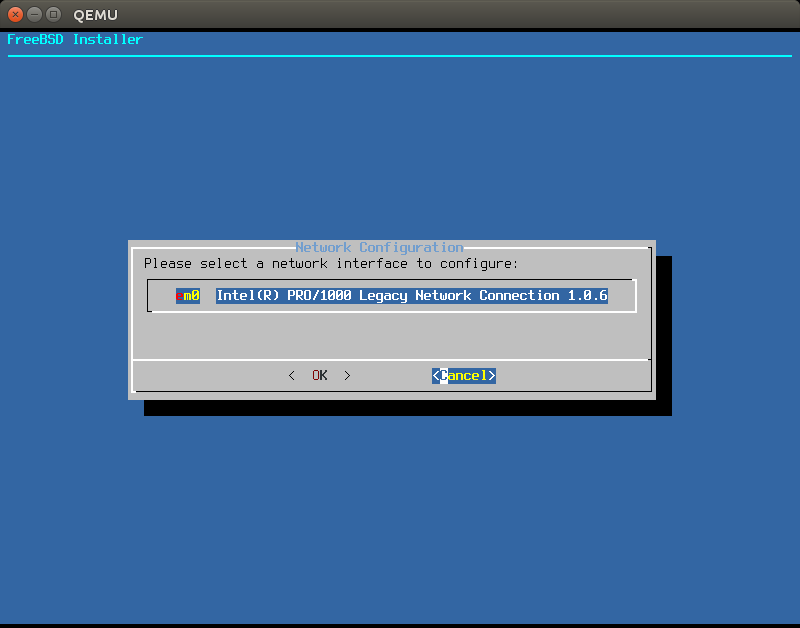
\includegraphics[width=10cm]{./IMG/FreeBSD_NIC.png}
	\end{center}
    \caption{NIC設定画面}
    \label{fig:FreeBSD_NIC}
\end{figure*}

タイムゾーンの設定を行います。
\ref{fig:FreeBSD_TIM}にて``$<$No$>$''を選択後、
\ref{fig:FreeBSD_TIM2}の国を選ぶリストで``18 Japan''を選択する。
\begin{figure*}[htbp]
	\begin{center}
    	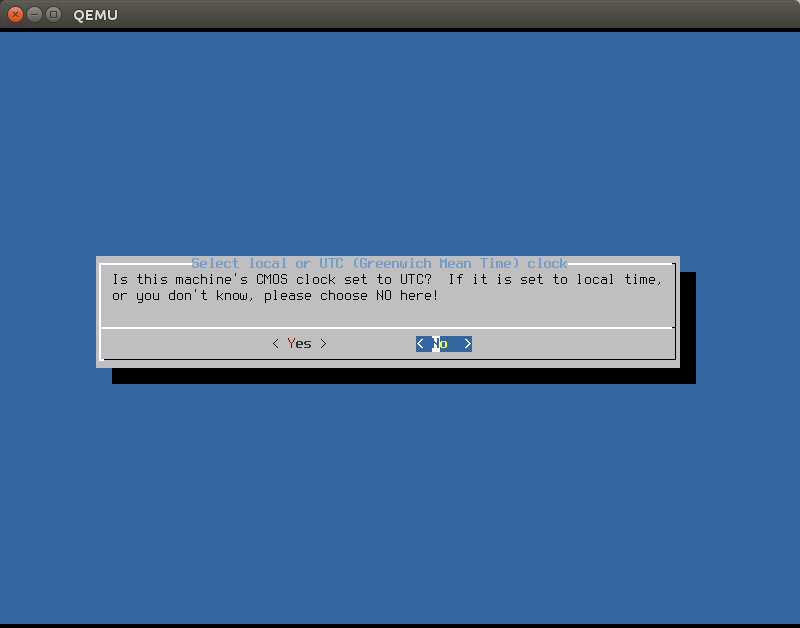
\includegraphics[width=10cm]{./IMG/FreeBSD_TIM.png}
	\end{center}
    \caption{タイムゾーン設定1}
    \label{fig:FreeBSD_TIM}
\end{figure*}
\begin{figure*}[htbp]
	\begin{center}
    	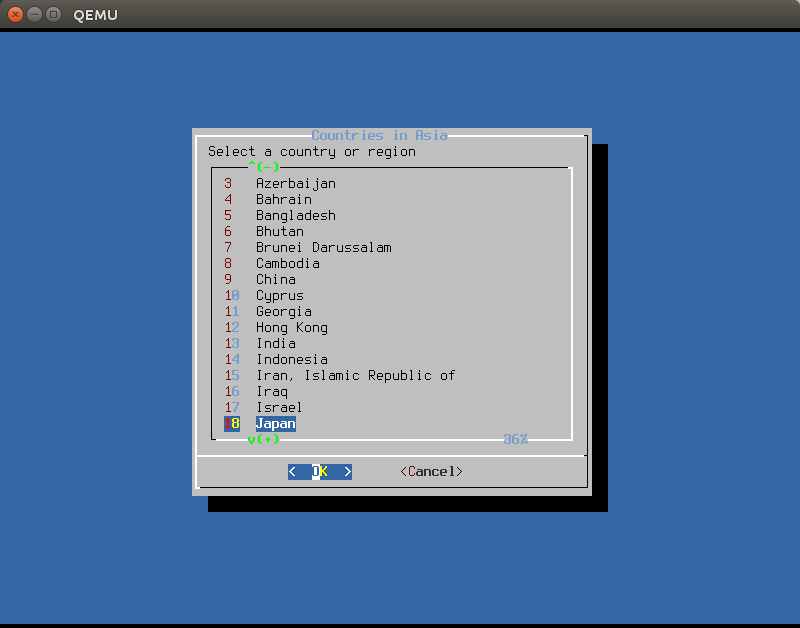
\includegraphics[width=10cm]{./IMG/FreeBSD_TIM_JP.png}
	\end{center}
    \caption{タイムゾーン設定2}
	\label{fig:FreeBSD_TIM2}
\end{figure*}

\ref{fig:FreeBSD_Service}で有効にするサービスを選ぶ。
筆者はsshdを無効にしているが、特に初期値でも問題ない。
\begin{figure*}[htbp]
	\begin{center}
    	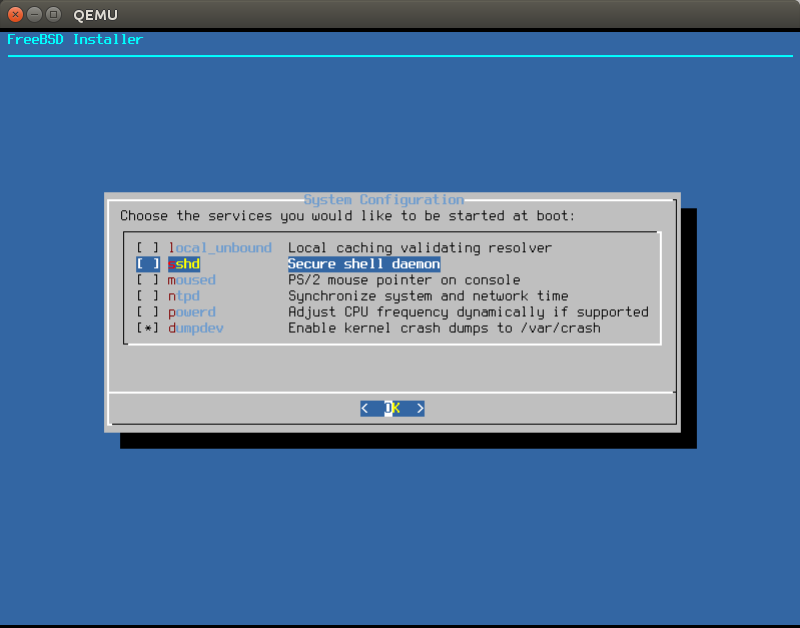
\includegraphics[width=10cm]{./IMG/FreeBSD_SYS.png}
	\end{center}
    \caption{FreeBSDで実行するサービス}
    \label{fig:FreeBSD_Service}
\end{figure*}

\ref{fig:FreeBSD_ADD_U}にて一般ユーザの追加えるが、
デバッガで一般ユーザをいれる理由もないので筆者は``$<$No$>$''を選択した。
\begin{figure*}[htbp]
	\begin{center}
    	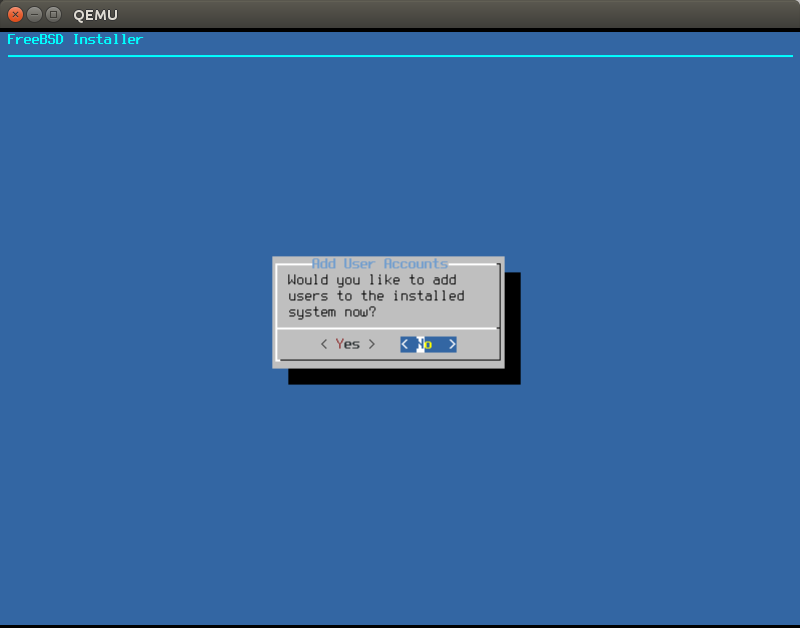
\includegraphics[width=10cm]{./IMG/FreeBSD_ADD_USER.png}
	\end{center}
    \caption{一般ユーザ追加}
    \label{fig:FreeBSD_ADD_U}
\end{figure*}
\clearpage

以降はインストールの完了作業である。
\ref{fig:FreeBSD_FIN_1}にて``Exit''を選択し、
\ref{fig:FreeBSD_FIN_2}にて``$<$No$>$''を選択し、
\ref{fig:FreeBSD_FIN_3}にて``$<$Reboot$>$''を選択すれば
インストールが完了してリブートする。
リブートが完了したら、一旦QEMUを終了させる。
\begin{figure*}[htbp]
	\begin{center}
    	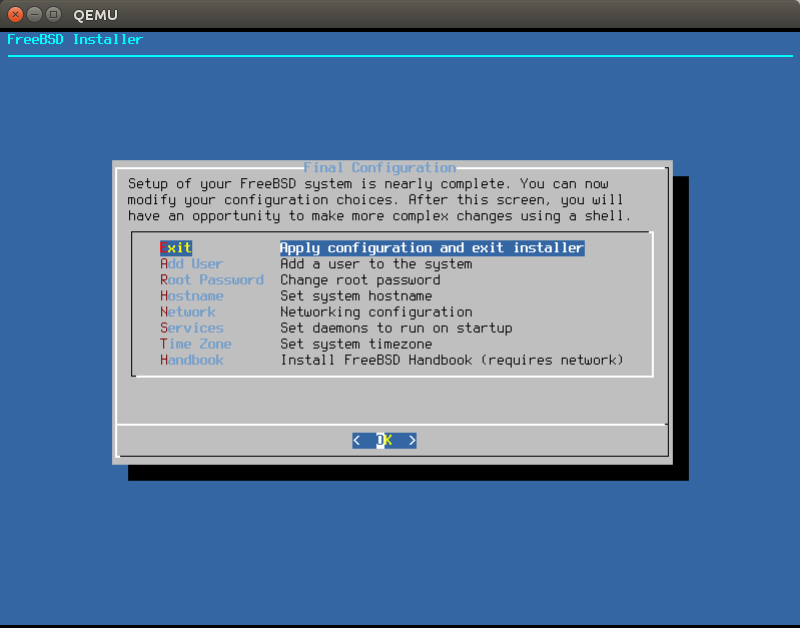
\includegraphics[width=10cm]{./IMG/FreeBSD_FIN.png}
	\end{center}
    \caption{FreeBSDインストール完了1}
    \label{fig:FreeBSD_FIN_1}
\end{figure*}
\begin{figure*}[htbp]
	\begin{center}
    	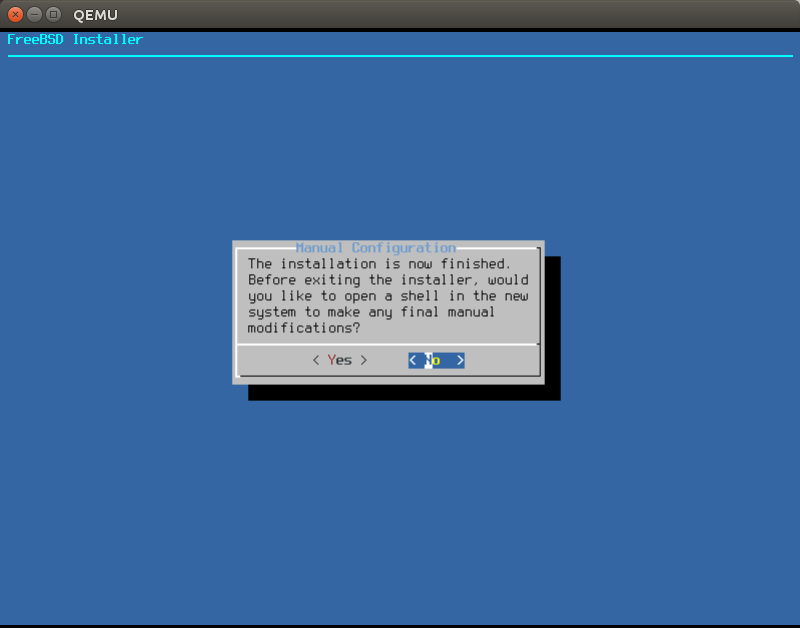
\includegraphics[width=10cm]{./IMG/FreeBSD_LST.png}
	\end{center}
    \caption{FreeBSDインストール完了2}
    \label{fig:FreeBSD_FIN_2}
\end{figure*}
\begin{figure*}[htbp]
	\begin{center}
    	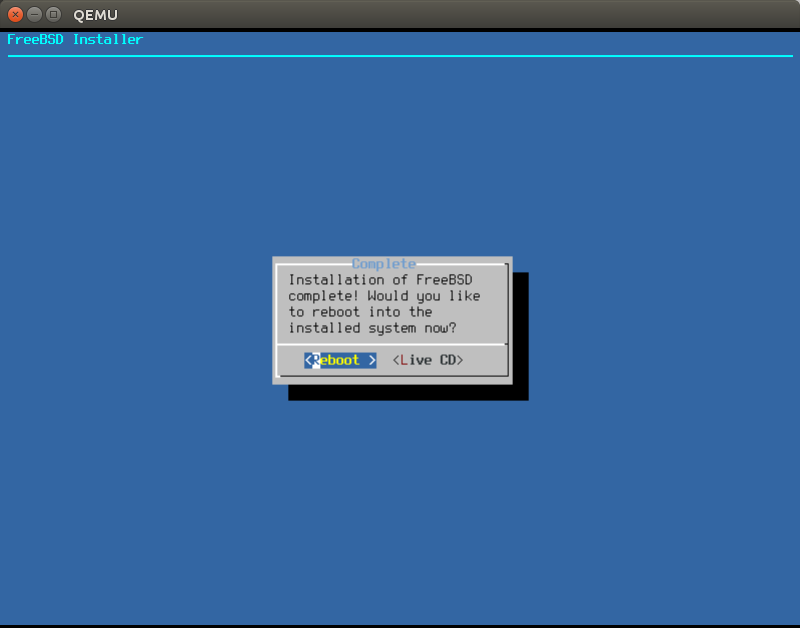
\includegraphics[width=10cm]{./IMG/FreeBSD_ALL_LAS.png}
	\end{center}
    \caption{FreeBSDインストール完了3}
    \label{fig:FreeBSD_FIN_3}
\end{figure*}


\subsection{Kernelの再構築のためのファイル編集}
\ref{sec:FreeBSD_inst}でインストールしたFreeBSDをデバッグできるようにKernelを再構築する。

\ref{fig:FreeBSD_boot_com}のコマンドでQEMUを起動してください。
\begin{figure*}[htbp]
	\begin{center}
		\begin{lstlisting}[basicstyle=\ttfamily\footnotesize, frame=single, breaklines=true]
$ qemu-system-x86_64 -enable-kvm -bios OVMF.fd -hda GUEST1 -m 1024M -smp 2
	    \end{lstlisting}
	\end{center}
	\caption{FreeeBSDを仮想ストレージから起動}
	\label{fig:FreeBSD_boot_com}
\end{figure*}

インストールできている場合は、しばらく経つと\ref{fig:FreeBSD_BOOT}の画面になります。
\begin{figure*}[htbp]
	\begin{center}
    	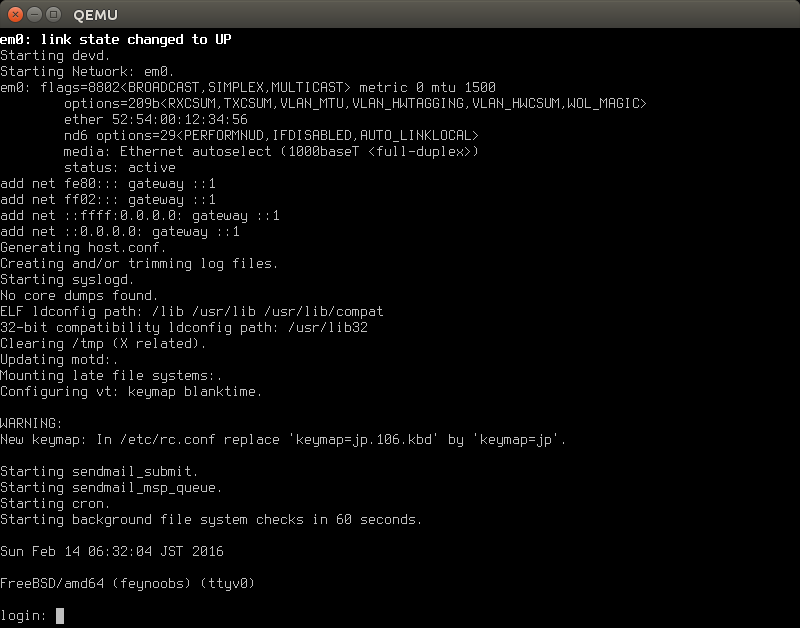
\includegraphics[width=10cm]{./IMG/FreeBSD_BOOT.png}
	\end{center}
    \caption{FreeBSD起動画面}
    \label{fig:FreeBSD_BOOT}
\end{figure*}

ログイン後3つのファイルを編集します。
なおFreeBSDインストール完了時には``vi''と``ee''の2つのエディタが組み込まれています。
筆者のように``vi''が苦手な者は、``ee''が直感的に使いやすいと思う。
\begin{itemize}
    \item /boot/device.hints
    \item /sys/amd64/conf/GENERIC.hints
    \item /sys/amd64/conf/GENERIC
\end{itemize}

\subsubsection{device.hintsの編集}
\label{sec:FreeBSD_device.hints}
device.hintsの中に\ref{fig:FreeBSD_bf_hints}の行がある。
この行を\ref{fig:FreeBSD_af_hints}に書き換えてエディタを閉じる。
\begin{figure*}[htbp]
	\begin{center}
		\begin{lstlisting}[basicstyle=\ttfamily\footnotesize, frame=single, breaklines=true]
hint.uart.0.flags="0x10"
		\end{lstlisting}
	\end{center}
	\caption{hints編集前}
	\label{fig:FreeBSD_bf_hints}
\end{figure*}

\begin{figure*}[htbp]
	\begin{center}
		\begin{lstlisting}[basicstyle=\ttfamily\footnotesize, frame=single, breaklines=true]
hint.uart.0.flags="0x90"
		\end{lstlisting}
	\end{center}
	\caption{hints編集後}
	\label{fig:FreeBSD_af_hints}
\end{figure*}

\subsubsection{GENERIC.hintsの編集}
device.hintsと全く同じなので割愛する。

\subsubsection{GENERICの編集}
GENERICの適当な場所に\ref{fig:FreeBSD_GENERIC}の内容を追記する。
\begin{figure*}[htbp]
	\begin{center}
		\begin{lstlisting}[basicstyle=\ttfamily\footnotesize, frame=single, breaklines=true]
options     DDB
options     GDB
		\end{lstlisting}
	\end{center}
	\caption{GENERICの編集}
	\label{fig:FreeBSD_GENERIC}
\end{figure*}

\subsection{Kernelの再構築実行}
\label{sec:Kern_build}
``/sys/amd64/conf''にて\ref{fig:FreeBSD_cf}を実行する。
そうすると、``/sys/amd64/compile/GENERIC''配下にKernelのソースコードが生成される。
これをコンパイルすることで新しいデバッグ用のKernelを作ることができる。
\begin{figure*}[htbp]
	\begin{center}
		\begin{lstlisting}[basicstyle=\ttfamily\footnotesize, frame=single, breaklines=true]
$ config GENERIC
		\end{lstlisting}
	\end{center}
	\caption{configファイルコンパイル}
	\label{fig:FreeBSD_cf}
\end{figure*}

コンパイルは\ref{fig:FreeBSD_kern}で実行する。
エラーなく終わればデバッグ用Kernelが生成されインストールされている。
ここまでで、一度シャットダウンする。
\begin{figure*}[htbp]
	\begin{center}
		\begin{lstlisting}[basicstyle=\ttfamily\footnotesize, frame=single, breaklines=true]
$ make cleandepend && make depend && make && make install
		\end{lstlisting}
	\end{center}
	\caption{Kernelコンパイル}
	\label{fig:FreeBSD_kern}
\end{figure*}

\section{Kernelデバッグ開始}

\newpage
\end{multicols}

\end{document}
